\documentclass[12pt, twoside]{article}
\usepackage[letterpaper, margin=1in, headsep=0.5in]{geometry}
\usepackage[english]{babel}
\usepackage[utf8]{inputenc}
\usepackage{amsmath}
\usepackage{amsfonts}
\usepackage{amssymb}
\usepackage{tikz}
%\usetikzlibrary{quotes, angles}

\usepackage{graphicx}
\usepackage{enumitem}
\usepackage{multicol}

\usepackage{fancyhdr}
\pagestyle{fancy}
\fancyhf{}
\renewcommand{\headrulewidth}{0pt} % disable the underline of the header

\fancyhead[RE]{\thepage}
\fancyhead[RO]{\thepage \\ Name: \hspace{3cm}}
\fancyhead[L]{BECA / Dr. Huson / 10th Grade Geometry\\* Unit 7: Analytic Geometry Review\\26 February 2019}

\begin{document}
\subsubsection*{7-16 Pre-test: Applying Algebra to Geometric Situations}
  \begin{enumerate}

  \item Write down the slope perpendicular to the given slope. \vspace{0.5cm}
    \begin{enumerate}
      \begin{multicols}{2}
      \item   $m= \frac{3}{2} \hspace{1cm} m_{\perp} = $ \vspace{1cm}
      \item   $m= -4 \hspace{1cm} m_{\perp} = $
      \item   $m= 0.25 \hspace{1cm} m_{\perp} = $ \vspace{1cm}
      \item   $m= -\frac{1}{3} \hspace{1cm} m_{\perp} = $
      \end{multicols}
    \end{enumerate}

  \item The line $l$ has the equation $y=2 x-5$.
  \begin{enumerate}
    \item What is the slope of the line $k$, given $k \parallel l$?
    \vspace{1cm}
    \item What is the slope of the line $m$, given $m \perp l$?
    \vspace{1cm}
  \end{enumerate}

  In the following problems, use the point-slope formula: $y-y_A=m (x-x_A)$
    \item What is the equation of a line through the point $A(5,-1)$ and parallel to the line $y=x-5$?  \vspace{2cm}

    \item \emph{Spicy} What is an equation of the perpendicular bisector of $\overline{QR}$ with $Q(5,-3)$ and $R(1,5)$? \vspace{5cm}


 \newpage

  \item Simplify each expression. (Leave it in radical form if necessary, not a decimal.)
    \begin{enumerate}
      \begin{multicols}{2}
      \item   $\sqrt{49}$ \vspace{1cm}
      \item   $\sqrt{20}$
      \item   $\sqrt{75}$ \vspace{1cm}
      \item   $\sqrt{\frac{1}{16}}$
      \end{multicols}
    \end{enumerate}
    \vspace{0.5cm}


  \item Write down the center and radius of each circle.
    \begin{enumerate}
      \begin{multicols}{2}
      \item   $(x-6)^2+y^2=36$ \vspace{2cm}
      \item   $(x+2)^2+(y+1)^2=18$
      \item   $(x-1)^2+(y-9)^2=7^2$ \vspace{2cm}
      \item   $(x+3)^2+(y-4)^2=18$
      \end{multicols}
    \end{enumerate}  \vspace{2cm}

  \item In the quadratic function below, a constant value, $p$, ``completes the square".

    \[f(x) = x^2+6x+p-p\]

    \begin{enumerate}
      \item What value of $p$ would complete the square? \vspace{1cm}
      \item Rewrite the function $f$ in vertex form. \vspace{3cm}
      \item Write down the value of the vertex of the graph of $f$ as a coordinate pair.  \vspace{2cm}
    \end{enumerate}

\newpage

  \item Graph and label the two equations. Mark their intersection as an ordered pair.

    \begin{multicols}{2}
      $y = \frac{3}{2}x-8$ \\
      $2x+6y = 18$
    \end{multicols}
    \vspace{1.5cm}

      \begin{center} %4 quadrant regents grid w T-Chart
      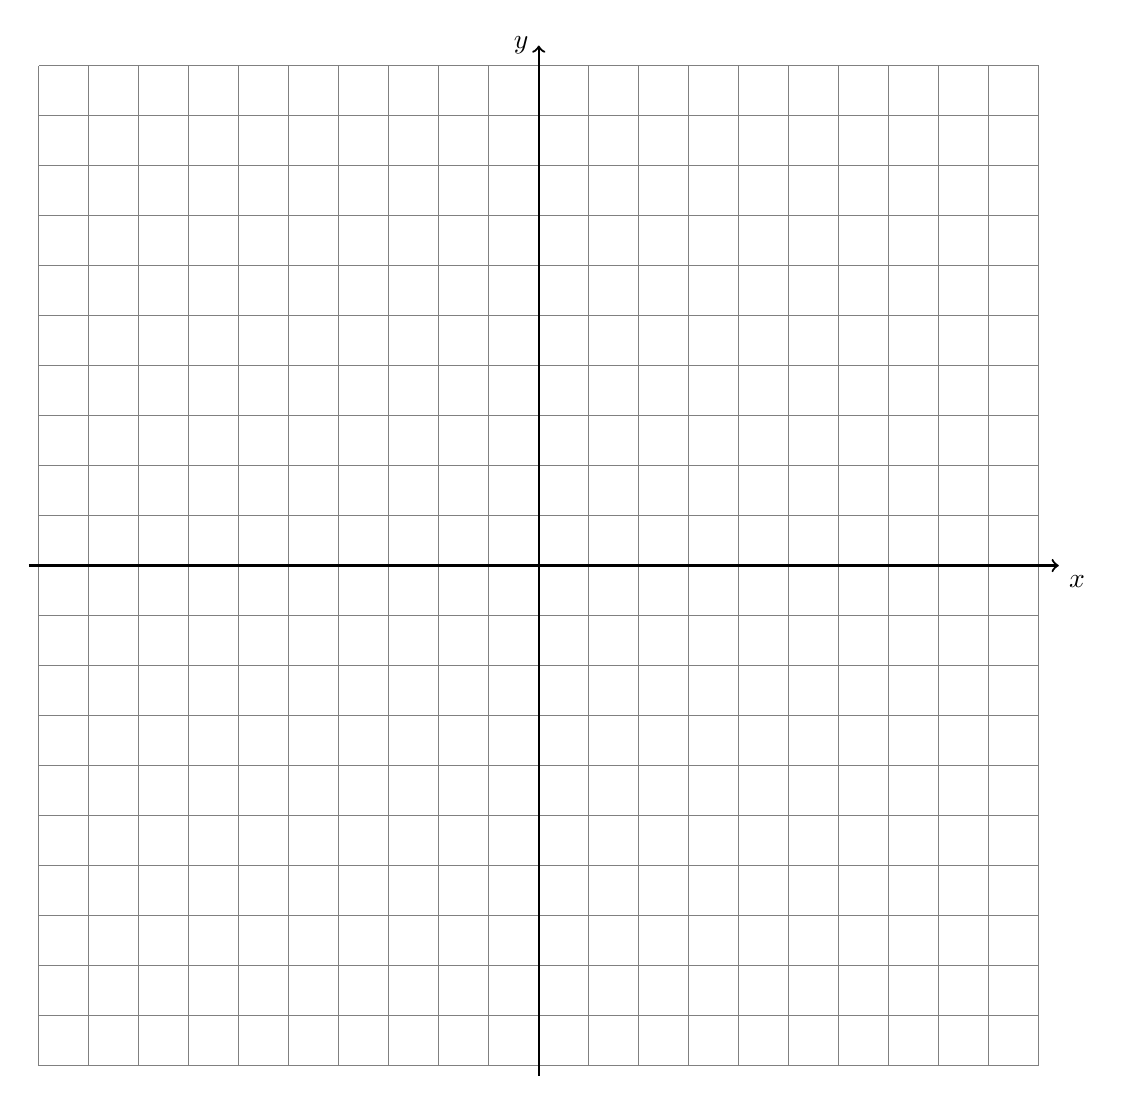
\begin{tikzpicture}[scale=.635]
        \draw [help lines] (-10,-10) grid (10,10);
        \draw [thick, ->] (-10.2,0) -- (10.4,0) node [below right] {$x$};
        \draw [thick, ->] (0,-10.2)--(0,10.4) node [left] {$y$};
      \end{tikzpicture}
      \end{center}
    Are the lines parallel, perpendicular, or neither? Justify your answer, stating the values of the lines' slopes.


\newpage

  \item Given $J(2,6)$ and $K(-1,3)$, find the length of $\overline{JK}$. Leave the result in simplified radical form (not a decimal).
      \vspace{4cm}

  \item On the graph below, draw $\overline{AB}$, with $A(-2,-1)$ and $B(4,7)$, labeling the end points.\\
    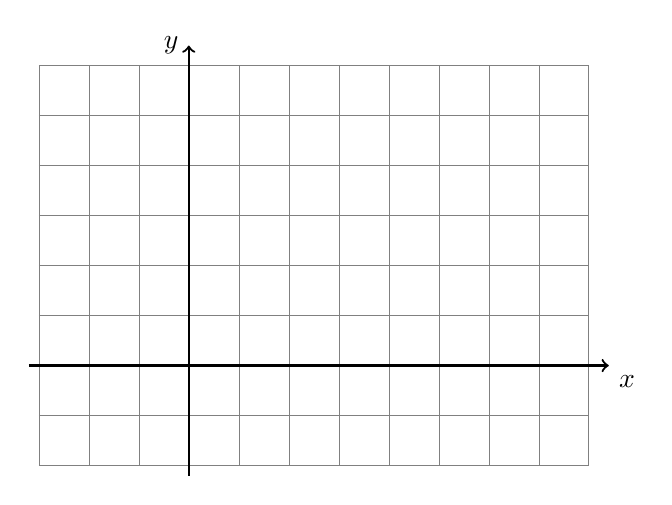
\begin{tikzpicture}[scale=.635]
      \draw [help lines] (-3,-2) grid (8,6);
      \draw [thick, ->] (-3.2,0) -- (8.4,0) node [below right] {$x$};
      \draw [thick, ->] (0,-2.2)--(0,6.4) node [left] {$y$};
    \end{tikzpicture}
    \begin{enumerate}
      \item Determine and state the coordinates of the midpoint $M$ of $\overline{AB}$. Mark $M$ and label it on the graph. \vspace{2cm}
      \item Find the slope of $\overline{AB}$. \vspace{2.5cm}
      \item Find the length of $\overline{AB}$.
    \end{enumerate}

\newpage

  \item In the diagram below, $\overline{AC}$ has endpoints with coordinates $A(-6,5)$ and $C(8, -2)$.
    \begin{center} %4 quadrant regents grid
      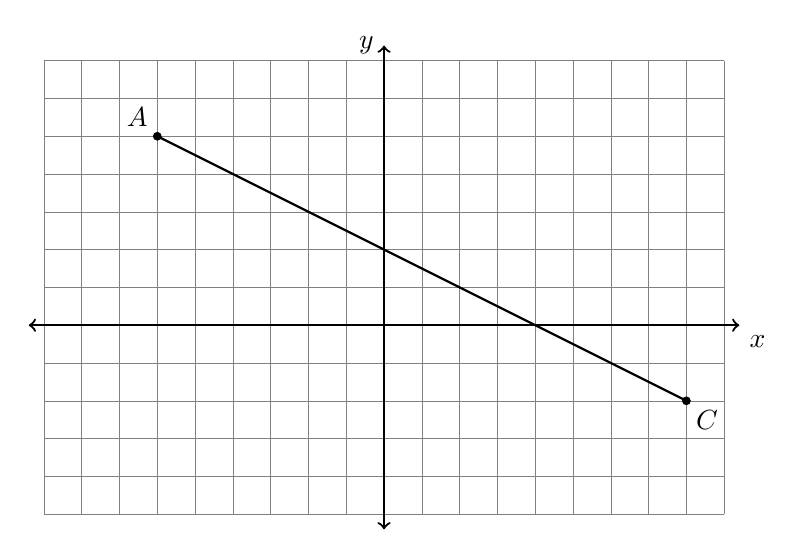
\begin{tikzpicture}[scale=.48]
        \draw [help lines] (-9,-5) grid (9,7);
        \draw [thick, <->] (-9.4,0) -- (9.4,0) node [below right] {$x$};
        \draw [thick, <->] (0,-5.4)--(0,7.4) node [left] {$y$};
        \draw [thick] (-6,5)--(8, -2);
        \draw [fill] (-6,5) circle [radius=0.1] node[above left] {$A$};
        \draw [fill] (8, -2) circle [radius=0.1] node[below right] {$C$};
      \end{tikzpicture}
    \end{center}
    If $B$ is a point on $\overline{AC}$ and $AB {:} BC = 4{:}3$,  what  are  the coordinates of $B$? \vspace{4cm}

  \item $A(-2,5)$ is one endpoint of $\overline{AB}$. The segment's midpoint is $M(3,3)$. Find the other endpoint, $B$. \vspace{3cm}

  \item A translation maps $A(-2,4) \rightarrow A'(-5,7)$. What is the image of $B(1,-3)$ under the same translation?  \vspace{3cm}

\newpage

  \item Given right $\triangle JKL$ with $\overline{JK} \perp \overline{KL}$, $JL=7.8$, $m\angle J=33^\circ$. Find the length $JK$, \emph{rounded to the nearest hundredth}.
    \begin{center}
      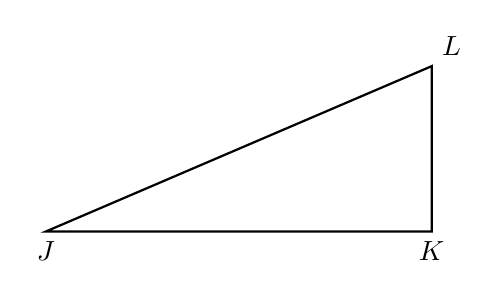
\begin{tikzpicture}[scale=0.7]
        \draw [thick]
        (0,0) node[below]{$J$}--
        (7,0)  node[below]{$K$}--
        (7,3) node[above right]{$L$}--cycle;
      \end{tikzpicture}
    \end{center}
\vspace{1cm}

  In the following two problems, solve for the value of $x$.
  \begin{multicols}{2}
  \item   $\frac{1}{4}(7x+5)=3$ \vspace{4cm}
  \item   $\frac{4}{3}(6-3x)=4$ \vspace{4cm}
  \end{multicols}

\vspace{3cm}

  \item Given $f(x)=\frac{3}{2} x+2$. Solve for $x$ such that for $f(x)=5$. \vspace{3.5cm}
  \item Given $g(x)=-x^2-7x-6$. Simplify $g(-1)$. \vspace{2cm}
  \item Given $h(x)=x^2+x-6$. Solve $h(x)=0$. \vspace{3cm}

\newpage

  \item Given triangle $ABC$ with $D$ the midpoint of $\overline{AB}$ and $E$ the midpoint of $\overline{AC}$, as shown. Given $AD=8$, $BD=x+4$, $DE=12$, and $BC=y+10$. \\[0.25cm] Find $x$ and $y$. \vspace{1cm}
    \begin{center}
        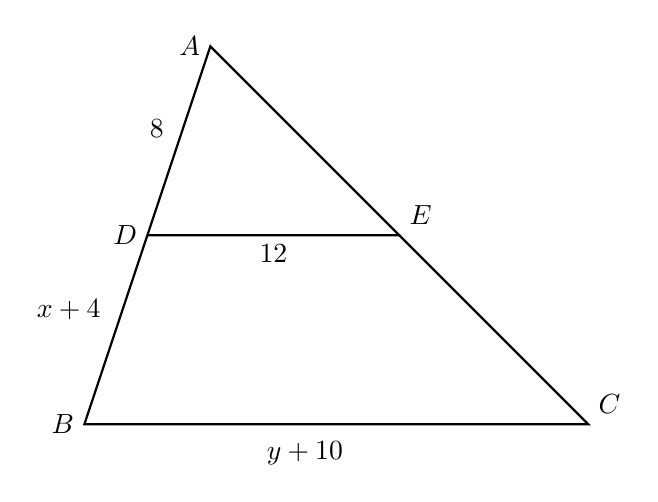
\begin{tikzpicture}[scale=0.4]
          \draw [thick]
          (0,0)node[left]{$D$}--
          (8,0)node[above right]{$E$}--
          (2,6)node[left]{$A$}--cycle;
          \draw [thick]
          (0,0)--
          (-2,-6)node[left]{$B$}--
          (14,-6)node[above right]{$C$}--(8,0);
          \node at (4,0)[below]{$12$};
          %\node at (5.3, 3)[right]{$7$};
          \node at (0.3, 2.8)[above]{$8$};
          \node at (-2.5, -3)[above]{$x+4$};
          \node at (5, -7.6)[above]{$y+10$};
        \end{tikzpicture}
      \end{center}
\vspace{1cm}

 \item Given $\triangle ABP$ and $\triangle JKP$ as shown below. $\overline{AB} \parallel \overline{JK}$. $AP=3.8$, $JP=9.5$, and $JK=16.5$. Find $AB$.\\[0.5cm]
   \begin{tikzpicture}[scale=1.4]
       \draw [thick]
         (0.25,-1)node[right]{$B$}--
         (-0.5,2)node[left]{$K$}--
         (4,0)node[right]{$J$}--
         (0,0)node[above right]{$P$}--
         (-2,0)node[left]{$A$}--cycle;
     \end{tikzpicture}


  \newpage


      \item Given the circle $C$ with circumference $8\pi$.
    \begin{enumerate}
      \item Write down the formula for the circumference of a circle and solve for the radius yielding a circumference of $8\pi$. \vspace{1cm}
      \item Find the area of the circle.
    \end{enumerate}
    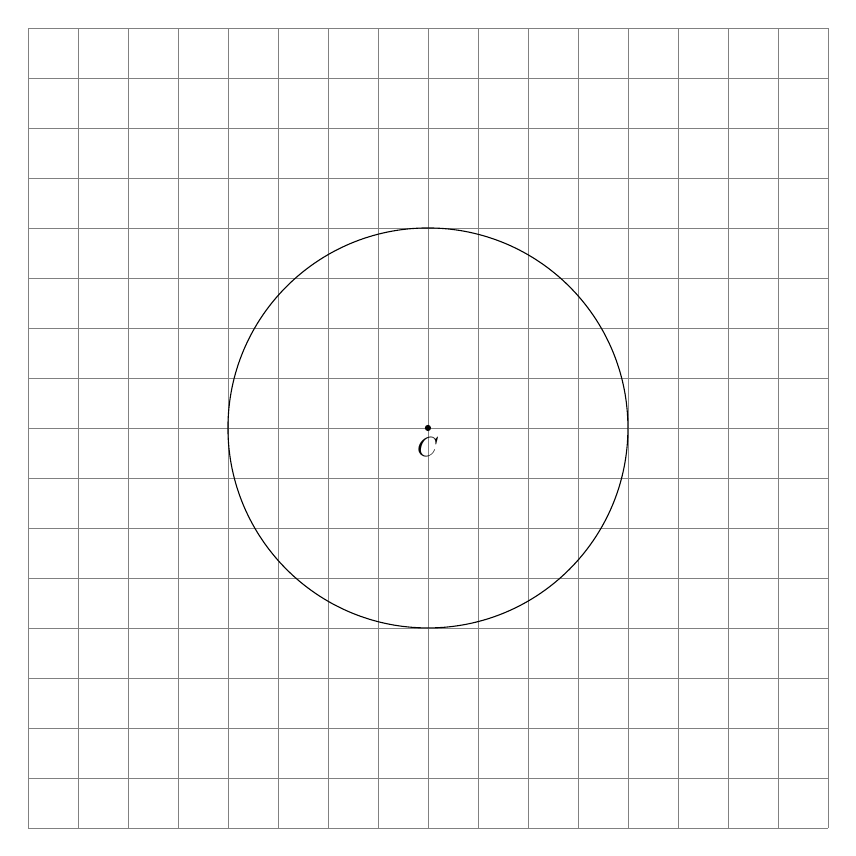
\begin{tikzpicture}[scale=.635]
      \draw [help lines] (-8,-8) grid (8,8);
      %\draw [thick, ->] (-2.2,0) -- (10.4,0) node [below right] {$x$};
      %\draw [thick, ->] (0,-2.2)--(0,10.4) node [left] {$y$};
      \draw (0,0) circle [radius=4] node[below]{$C$};
      \draw [fill] (0,0) circle [radius=0.05];
    \end{tikzpicture}

    \item Given a circle $O$ with radius $5$.
    \begin{enumerate}
      \item Find the circumference of $O$. \vspace{2cm}
      \item Find the area of $O$. \vspace{2cm}
    \end{enumerate}



  \end{enumerate}

  \end{document}
